

STL使用迭代器来导航其容器类的元素,大多数容器都包含begin()和end()迭代器,通常实现为返回迭代器对象的成员函数。begin()迭代器指向容器的初始元素,end()迭代器指向最终元素之后的元素:

\hspace*{\fill} \\ %插入空行
\begin{center}
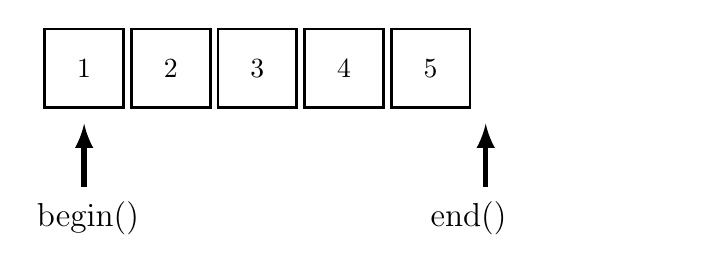
\begin{tikzpicture}
\foreach \x in {1,...,5} {
	\draw[line width=1pt] (1.1*\x,1) rectangle (1.1*\x+1,0) node[pos=.5] {\x};
}

\draw[line width=2pt][-latex] (1.6,-1.0) -- (1.6,-0.2);
\draw[line width=2pt][-latex] (6.7,-1.0) -- (6.7,-0.2);

\node[text width=3cm, font=\large] at (2.5,-1.4) {begin()};
\node[text width=3cm, font=\large] at (7.5,-1.4) {end()};
\end{tikzpicture}

图4.1  begin()和end()迭代器
\end{center}

end()迭代器可以作为长度不确定的容器的哨兵。我们将在本章中看到一些例子。

大多数STL容器都定义了自己特定的迭代器类型。例如,对于int类型的vector:

\begin{lstlisting}[style=styleCXX]
std::vector<int> v;
\end{lstlisting}

迭代器类型定义为:

\begin{lstlisting}[style=styleCXX]
std::vector<int>::iterator v_it;
\end{lstlisting}

可以看到这是多么复杂。若有一个string的vector

\begin{lstlisting}[style=styleCXX]
std::vector<std::vector<int, std::string>> v;
\end{lstlisting}

其迭代器类型为:

\begin{lstlisting}[style=styleCXX]
std::vector<std::vector<int, std::string>>::iterator v_it;
\end{lstlisting}

幸运的是,C++11提供了auto类型推断和自动类型。通过使用auto,很少需要使用完整的迭代器类型定义。例如,在for循环中需要迭代器,可以使用auto类型:

\begin{lstlisting}[style=styleCXX]
for(auto v_it = v.begin(); v_it != v.end(); ++v_it) {
	cout << *v_it << '\n';
}
\end{lstlisting}

注意使用解引用操作符从迭代器中访问元素,这和解引用指针的语法一样:

\begin{lstlisting}[style=styleCXX]
const int a[]{ 1, 2, 3, 4, 5 };
size_t count{ sizeof(a) / sizeof(int) };
for(const int* p = a; count > 0; ++p, --count) {
	cout << *p << '\n';
}
\end{lstlisting}

可以使用一个基于范围的for循环和一个原生数组:

\begin{lstlisting}[style=styleCXX]
const int a[]{ 1, 2, 3, 4, 5 };
for(auto e : a) {
	cout << e << '\n';
}
\end{lstlisting}

或者使用STL容器:

\begin{lstlisting}[style=styleCXX]
std::vector<int> v{ 1, 2, 3, 4, 5 };
for(auto e : v) {
	cout << e << '\n';
}
\end{lstlisting}

基于范围的for循环只是带迭代器的for循环的简写:

\begin{lstlisting}[style=styleCXX]
{
	auto begin_it{ std::begin(container) };
	auto end_it{ std::end(container) };
	for ( ; begin_it != end_it; ++begin_it) {
		auto e{ *begin_it };
		cout << e << '\n';
	}
}
\end{lstlisting}

因为迭代器使用与基元指针相同的语法,所以基于范围的for循环对这两种容器的处理都一样。

注意,基于范围的for循环调用std::begin()和std::end(),而不是直接调用begin()和end()成员函数。函数调用成员函数来获取迭代器。为什么不直接调用成员函数呢?非成员函数也设计用于原始数组。这就是为什么for循环适用于数组:

\begin{lstlisting}[style=styleCXX]
const int arr[]{ 1, 2, 3, 4, 5 };
for(auto e : arr) {
	cout << format("{} ", e);
}
\end{lstlisting}

输出为:

\begin{tcblisting}{commandshell={}}
1 2 3 4 5
\end{tcblisting}

通常,我倾向于使用成员函数begin()和end(),因为它们更显式。其他人更喜欢使用std::的非成员函数,因为它们更通用。萝卜白菜,各有所爱;不过,我建议读者们选择一种风格并坚持下去。

\subsubsection{类别}

C++20之前,迭代器根据其功能分为以下几类:

% Please add the following required packages to your document preamble:
% \usepackage{multirow}
\begin{table}[H]
\centering
\begin{tabular}{|llllll|}
\hline
\multicolumn{5}{|c|}{\textbf{迭代器类别}} &
\multicolumn{1}{c|}{\textbf{迭代器功能}} \\ \hline
\multicolumn{1}{|l|}{\multirow{5}{*}{\begin{tabular}[c]{@{}l@{}}连续\\ 迭代器\end{tabular}}} &
\multicolumn{1}{l|}{\multirow{4}{*}{\begin{tabular}[c]{@{}l@{}}随机\\ 访问迭代器\end{tabular}}} &
\multicolumn{1}{l|}{\multirow{3}{*}{\begin{tabular}[c]{@{}l@{}}双向\\ 迭代器\end{tabular}}} &
\multicolumn{1}{l|}{\multirow{2}{*}{\begin{tabular}[c]{@{}l@{}}前向\\ 迭代器\end{tabular}}} &
\multicolumn{1}{l|}{输入迭代器} &
\begin{tabular}[c]{@{}l@{}}·读取\\ ·递增一次\end{tabular} \\ \cline{5-6} 
\multicolumn{1}{|l|}{} &
\multicolumn{1}{l|}{} &
\multicolumn{1}{l|}{} &
\multicolumn{1}{l|}{} &
\multicolumn{1}{l|}{} &
·递增多次 \\ \cline{4-6} 
\multicolumn{1}{|l|}{} &
\multicolumn{1}{l|}{} &
\multicolumn{1}{l|}{} &
\multicolumn{2}{l|}{} &
·可递减 \\ \cline{3-6} 
\multicolumn{1}{|l|}{} &
\multicolumn{1}{l|}{} &
\multicolumn{3}{l|}{} &
·随机访问 \\ \cline{2-6} 
\multicolumn{1}{|l|}{} &
\multicolumn{4}{l|}{} &
·连续存储 (比如数组) \\ \hline
\multicolumn{6}{|l|}{当上面任何一个迭代器也可以写入时,也称为可变迭代器。} \\ \hline
\multicolumn{5}{|l|}{输出迭代器} &
\begin{tabular}[c]{@{}l@{}}·可写入\\ ·递增一次\end{tabular} \\ \hline
\end{tabular}
\end{table}

这些类别是分层级的,功能较强的迭代器继承功能较弱的迭代器的功能,输入迭代器只能读取和递增一次。前向迭代器具有输入迭代器的功能,并且可以多次递增。双向迭代器具有这些功能,还可以自减。

输出迭代器可以写入和递增一次。若其他迭代器也可以写入,则是可变迭代器。

\subsubsection{概念}

C++20的概念和约束是新加入的特性。概念只是一个命名约束,将参数的类型限制在模板函数或类中,并帮助编译器选择适当的特化。

C++20起,STL用概念而不是类别来定义迭代器。这些概念都在std::命名空间中。

\begin{table}[H]
\centering
\begin{tabular}{|l|l|}
\hline
\textbf{概念} &
\textbf{描述} \\ \hline
indirectly\_readable &
\begin{tabular}[c]{@{}l@{}}迭代器可以由解引用操作符读取。\\ 这包括指针、智能指针和输入迭代器。\end{tabular} \\ \hline
indirectly\_writeable &
迭代器的对象引用是可写的。 \\ \hline
weakly\_incrementable &
\begin{tabular}[c]{@{}l@{}}这个值可以用++递增,但不能保持相等。\\ 例如,a==b,但++a可能不等于++b。\end{tabular} \\ \hline
incrementable &
可以用++增加,并且保持相等。 \\ \hline
\begin{tabular}[c]{@{}l@{}}input\_or\_output\_\\ iterator\end{tabular} &
\begin{tabular}[c]{@{}l@{}}迭代器可以递增和解引用。\\ 每个迭代器都必须满足这个概念。\end{tabular} \\ \hline
sentinel\_for &
\begin{tabular}[c]{@{}l@{}}哨兵迭代器用于查找大小不确定的对象的结束, \\ 例如输入流。\end{tabular} \\ \hline
sized\_sentinel\_for &
\begin{tabular}[c]{@{}l@{}}哨兵迭代器可以与另一个迭代器和-操作符一起使用,\\ 以确定它在常数时间内的距离。\end{tabular} \\ \hline
input\_iterator &
可读且可加的迭代器。 \\ \hline
output\_iterator &
可写入且可递增的迭代器。 \\ \hline
forward\_iterator &
这将使input\_iterator具有可递增性。 \\ \hline
\end{tabular}
\end{table}

\begin{table}[H]
\centering
\begin{tabular}{|l|l|}
\hline
\begin{tabular}[c]{@{}l@{}}bidirectional\_\\ iterator\end{tabular} &
\begin{tabular}[c]{@{}l@{}}它通过使用--操作符自减添加能力\\ preserves 来修改forward\_iterator,使其保持相等。\end{tabular} \\ \hline
\begin{tabular}[c]{@{}l@{}}random\_access\_\\ iterator\end{tabular} &
\begin{tabular}[c]{@{}l@{}}通过添加对+、+=、-、-=和{[}{]}操作符\\ 的支持对bidirectional\_iterator进行修改。\end{tabular} \\ \hline
contiguous\_iterator &
修改random\_access\_iterator以表示连续的存储。 \\ \hline
\end{tabular}
\end{table}

可以使用这些概念来约束模板的参数:

\begin{lstlisting}[style=styleCXX]
template<typename T>
requires std::random_access_iterator<typename T::iterator>
void printc(const T & c) {
	for(auto e : c) {
		cout << format("{} ", e);
	}
	cout << '\n';
	cout << format("element 0: {}\n", c[0]);
}
\end{lstlisting}

函数需要一个random\_access\_iterator。若用非随机访问容器的列表使用时,编译器会报错:

\begin{lstlisting}[style=styleCXX]
int main()
{
	list<int> c{ 1, 2, 3, 4, 5 };
	printc(c);
}
\end{lstlisting}

list迭代器类型不支持random\_access\_iterator概念。所以,编译器又报出了一个错误:

\begin{tcblisting}{commandshell={}}
error: no matching function for call to 'printc(std::__
cxx11::list<int>&)'
  27 | printc(c);
       | ~~~~~~^~~
note: candidate: 'template<class T> requires random_access_
iterator<typename T::iterator> void printc(const T&)'
  16 | void printc(const T & c) {
      |         ^~~~~~
note: template argument deduction/substitution failed:
note: constraints not satisfied
\end{tcblisting}

这是GCC的错误输出。不同编译器的错误看起来可能不同。

若用一个vector来调用,其是一个随机访问容器:

\begin{lstlisting}[style=styleCXX]
int main()
{
	vector<int> c{ 1, 2, 3, 4, 5 };
	printc(c);
}
\end{lstlisting}

现在编译和运行都挺好:

\begin{tcblisting}{commandshell={}}
$ ./working
1 2 3 4 5
element 0: 1
\end{tcblisting}

虽然针对不同类型的功能(和概念)有不同类型的迭代器,但其复杂性是为了支持易用性。

通过对迭代器的介绍,现在让我们继续本章中的主菜:

\begin{itemize}
\item 
创建可迭代范围

\item 
使迭代器与STL迭代器特性兼容

\item 
使用迭代器适配器填充STL容器

\item 
创建一个迭代器生成器

\item 
反向迭代器适配器的反向迭代

\item 
用哨兵迭代未知长度的对象

\item 
构建zip迭代器适配器

\item 
创建随机访问迭代器
\end{itemize}


